\chapter{Optimal Synthesis of Planar Four-bar Linkages for Extended Burmester Problem}\label{ExtendedBurmester}

\section{Introduction}
According to an article by Prof. McCarthy~\cite{McCarthy-blog}, over the past forty years, a total number of $2,688$ U.S. patents have been awarded that involve four-bar linkages, while in the same period, the next natural extension to more complex linkages, viz., six-bar linkages have been awarded a mere 84 patents.
This is a clear demonstration of the popularity and ubiquity of planar four-bar linkages. Therefore, it is not surprising that the four-bar linkage synthesis and analysis problem still receives a considerable attention of researchers.

Several text books, such McCarthy and Soh \cite{sohmccarthy}, Sandor and Erdman~\cite{Sandor}, Hunt \cite{Hunt78}, Hartenberg and Denavit \cite{Hartenberg},  Suh and Radcliffe \cite{Suh78}, and Lohse \cite{lohse2013} cover the science and art of planar four-bar and higher-order linkages.

Kerle et.al.\cite{modler2011} have given a historical overview of the development of mechanisms for motion generation.  Despite a glut of literature on this topic, simultaneous computation of type and dimensions and accommodating practical geometric constraint for the motion generation problem has not been explored much.
Erdman et al. in their seminal Mechanism Design and Analysis text~\cite{ErdmanSandor} clearly mention that assuming the wrong type (linkage topology and type of joints) to compute the dimensions of a linkage system may result in either none or sub-optimal solutions.

The work presented in this chapter is a continuation of our research~\cite{generalfitting-JCISE,motiongen-JMR,ge2012novel}, wherein we have presented a task-driven approach to simultaneous type and dimensional synthesis of planar dyads for the motion generation problem.
A four-bar linkage is constructed as combination of any two of the synthesized dyads.
This dyadic construction simplifies the synthesis process and renders the method as modular building block for synthesis of mechanisms with more links such as six-bar mechanisms \cite{generalfitting-JCISE}.
By using the concepts of kinematic mapping (Blaschke~\cite{Blaschke1911}, Gr{\"u}nwald~\cite{Grunwald1911}) and planar quaternions (Bottema and Roth~\cite{Bottema}, McCarthy~\cite{McCarthy90}), we obtained a unified form of kinematic constraints of the planar dyads and created an algorithm for unified type and dimensional synthesis of planar four-bar linkages. This is accomplished via a two-step process.
The first step is algebraic fitting of image points on a pencil of G-manifolds using Singular Value Decomposition (SVD).
This pencil of G-manifolds forms a candidate solution space for constraints accounted for in the SVD process.
In the second step, we impose two fundamental quadratic conditions on the candidate solutions to extract the dyad types and their dimensions.

Ravani and Roth~\cite{ravani83,ravani84} were the first to use kinematic mapping approach for mechanism synthesis.
Thereafter, Bodduluri and McCarthy \cite{Bodduluri92}, Bodduluri \cite{Bodduluri},  Ge and Larochelle \cite{GeLarochelle99}, Larochelle \cite{Larochelle, Larochelle1996}, Husty et al. \cite{Husty2007}, Hayes et al.~\cite{Hayes2004, Hayes2011}, Wu et al.~\cite{WuPurwarGe2010}, Purwar and Gupta~\cite{PurwarGupta2011}, and Shrocker et al.~\cite{schroker-planar} have used this approach for the motion generation problem.

The original contribution of the work presented in this chapter is in reformulation of the above framework in a general way so that classic Burmester problem can be extended to accommodate both pose- and other practical-geometric constraints, and so that it solves problems which our previous approach could not solve.
These problems are 1) finding optimal approximate solutions for Burmester problem with no or sub-optimal solutions, and  2) finding optimal linkages that minimize the algebraic fitting error of non-linear geometric constraints. We note that in this work, we do not restrict Burmester problem to only five poses.
Burmester~\cite{Burmester86} showed that only a finite set of four-bars can be synthesized for five precision pose motion generation problem. In this chapter, we show that other than poses, other practical geometric constraints can also be accommodated.
For more than five geometric constraints, typically only an approximate motion synthesis can be performed. Holte et al.\cite{holte2000}, Sabada et al. \cite{bawab1997}, Venkataraman\cite{Venkataraman1992}, have presented some techniques for mixed exact-approximate synthesis of planar mechanisms, albeit only for poses.
Larochelle\cite{Larochelle2015}  has presented dimensional synthesis technique for solving the mixed exact and approximate motion synthesis problem for planar RR kinematic chains.
Song~\cite{song2015} has presented Pole Curve Transformation based approach for motion synthesis of planar mechanisms.
Al-Widyan et al.\cite{Al-Widyan2002} have presented a numerically robust algorithm to solve the classic Burmester problem. Bourrelle et al.~\cite{bourrelle2007} presented a graphical user interface that uses the algorithm developed in~\cite{Al-Widyan2002} to solve the classic Burmester problem.

In general, there are two basic approaches to linkage synthesis for motion generation problem: 1) precision pose approach, and 2) error minimization approach. In this chapter, we use a combination of both methods in our framework.

Optimal synthesis of linkages is often a constrained non-linear and multi-modal problem in a multi-dimensional design space. In case of optimal linkage synthesis, relatively more work has been reported for path and function generation problem than for motion generation. Mariappan and Krishnamurty\cite{mariappan1996} used a generalized exact gradient method for planar mechanism synthesis. Vallejo\cite{vallejo1995} developed an optimization method for planar mechanisms with lower pairs of any type which uses error function as deformation of dimensions that mechanism has to undergo to perform the task. Yao and Angeles\cite{YaoAngeles2000} solved path-generation problem using least squared error function. They employ contour method to find out all stationery points of the problem. Kramer and Sandor~\cite{kramer1975} have presented a method of optimal design of planar mechanisms called Selective Precision Synthesis (SPS). SPS can incorporate design requirements such as link ratios, fixed pivot locations, and transmission angle range. Gogate and Matekar \cite{gogate2012} used method of differential evolution to find optimal linkages based on three error functions which ensure that the mechanism is crank rocker, branch and circuit defect free with minimized positional and angular deviations. Venkataraman et al.\cite{Venkataraman1992} used tolerance based approach for four position problem. They searched for optimal design parameters along suitable ranges of center point curve. Cabrera et al.\cite{Cabrera2002} have presented genetic algorithm on planar 4R mechanism synthesis for its simple implementation and fast convergence. Hegedus et al.~\cite{Hegedus2015} recently presented synthesis of spatial 6R linkages for interpolating four given poses using factorization of motion polynomials. All of the above said methods first select the type of linkage to be optimized, while our approach takes unified representation for all types of planar dyads into account. In contrast to other methods, which directly use linkage parameters, we formulate the optimization problem in terms of intermediate parameters obtained by geometric fitting. This allows us to use a two-step process wherein we first perform the least-squares fitting of the geometric constraints and then use a Lagrange multiplier method with additional linear and non-linear constraints to extract the dyad types and dimensions. This approach allows formulation of an objective function consisting of squared error for the constraints to be minimized, while keeping certain other constraints exactly satisfied. Ultimately, the minimization procedure leads to a system of quadratic equations, which can be solved using a Computer algebra softwares like Mathematica. Each real solution of this system of equation corresponds to one optimum dyad; all such dyads are computed and then combined pairwise to obtain a set of four-bar linkage solutions.

The organization of the chapter is as follows: Section~\ref{kinmap} reviews the concept of kinematic mapping and planar quaternions as a special case of dual quaternions. Section~\ref{gman} reviews unified form of kinematic constraints of the planar dyads as G-manifolds in the image space, while section~\ref{practConstraints} presents various geometric constraints in the image space. Section~\ref{algebraicFitting} presents how we  algebraically fit various linear geometric constraints to the G-manifolds using SVD. Section~\ref{optimality} presents the Lagrange Multiplier method to minimize error functions while keeping certain linear- or non-linear constraints satisfied exactly. We finally present two practical examples in section~\ref{examples}.

%%%%%%%%%%%%%%%%%%%%%%%%%%%%%%%%%%%%%%%%%%%%%%%%%%%%%%%%%%%%%%%%%%%%%%
\section{Kinematic Mapping}\label{kinmap}
A planar displacement consisting of a translation $(d_1,d_2)$ and a rotation  angle $\phi$ from a moving frame \textit{M} to a fixed frame \textit{F} is represented by a planar quaternion
 ${\bf Z}=(Z_1,Z_2,Z_3,Z_4)$ where (see \cite{ravani83,McCarthy90} for details),
\begin{equation}\label{z12}
\begin{array}{ll}
Z_1=\frac{1}{2}(d_1\cos\frac{\phi}{2}+d_2\sin\frac{\phi}{2}),  & Z_2=\frac{1}{2}(-d_1\sin\frac{\phi}{2}+d_2\cos\frac{\phi}{2}), \\
Z_3=\sin\frac{\phi}{2}, & Z_4= \cos\frac{\phi}{2}.
\end{array}
\end{equation}


The components $(Z_1,Z_2,Z_3,Z_4)$  define a point in a projective three-space called the {\it image space} of planar displacements~\cite{ravani83}.
Then, a planar displacement represented as a homogeneous transformation of point ${\bf x}=(x_1,x_2,x_3)$ or line  ${\bf l}=(l_1,l_2, l_3)$ from $M$ to $F$ can be given by
\begin{eqnarray}
{\bf X} &= &[H]{\bf x} \label{pointT}, \\ \nonumber \ \   [H] & = &\left[
\begin{array}{ccccc}
Z_4^2-Z_3^2 &  & -2Z_3Z_4 &  & 2(Z_1Z_3+Z_2Z_4) \\
2Z_3Z_4 &  & Z_4^2-Z_3^2 &  & 2(Z_2Z_3-Z_1Z_4) \\
0 &  & 0 &  & Z_3^2+Z_4^2
\end{array}
\right],\\
{\bf L} &=& [\overline{H}] {\bf l}\label{L2}, \\ \nonumber \ \  [\overline{H}] &=& \left[
\begin{array}{ccccc}
Z_4^2-Z_3^2 &  & -2Z_3Z_4 &  & 0\\
2Z_3Z_4 &  & Z_4^2-Z_3^2 &  & 0 \\
2(Z_1Z_3-Z_2Z_4)  & &  2(Z_2Z_3+Z_1Z_4)  & & Z_3^2+Z_4^2
\end{array}
\right],
\end{eqnarray}
where $Z_3^2+Z_4^2=1$ and ${\bf X}=(X_1,X_2,X_3)$ and ${\bf L}=(L_1,L_2,L_3)$ are corresponding point and line coordinates in $F$.

%%%%%%%%%%%%%%%%%%%%%%%%%%%%%%%%%%%%%%%%%%%%%%%%%%%%%%%%%%%%%%%%%%%%%%
\section{Generalized (G-) Constraint Manifold}\label{gman}
In this section, we review a unified form of the kinematic constraints of four types of dyads (\emph{RR}, \emph{PR}, \emph{RP}, and \emph{PP}) in the image space; see~\cite{generalfitting-JCISE} for details.
A point \textbf{X} or line \textbf{L} on the coupler of a four-bar linkage can be geometrically constrained in one of the following four ways: 1) for an \emph{RR} dyad, the point is constrained to be on a circle with center and radius given as homogeneous coordinates $(a_0,a_1,a_2, a_3)$,  2) for a \emph{PR} dyad, the point is constrained to be on a fixed line having coordinates $(L_1,L_2,L_3)$, 3) for an \emph{RP} dyad, a moving line $(l_1,l_2,l_3)$ is constrained to be tangent to a circle $(a_1,a_2,a_3)$, and 4) for \emph{PP} dyad, a point on line $(L_1,L_2,L_3)$ is constrained to move along another line $(2a_1,2a_2,a_3)$. In \cite{generalfitting-JCISE}, we have shown that all of these constraints reduce to a single quadratic equation in the Cartesian space. When the fixed frame coordinates of point and line from Eqns.~\req{pointT} and \req{L2} are substituted in this quadratic condition, we obtain following generalized equation:
\begin{eqnarray}\label{general}
& & p_1(Z_1^2+Z_2^2)+p_2(Z_1Z_3-Z_2Z_4)+p_3(Z_2Z_3+Z_1Z_4) \nonumber \\
& & \ \ \ \ \ \ \ \ \  + p_4(Z_1Z_3+Z_2Z_4) +p_5(Z_2Z_3-Z_1Z_4)+p_6Z_3Z_4 \nonumber \\ & & \ \ \ \ \ \ \ \ \ +p_7(Z_3^2-Z_4^2)+p_{8}(Z_3^2+Z_4^2)=0,
\end{eqnarray}
where the eight coefficients $p_i$ are not independent but must satisfy two quadratic conditions
\begin{equation}\label{2relation}
p_1p_6 +p_2p_5-p_3p_4 = 0 , \ \
2p_1p_7-p_2p_4 -p_3p_5 = 0.
\end{equation}
This is because   $p_i$ are related to the geometric parameters of the dyad by
\begin{equation}\label{8p}
\begin{array}{l}
p_1=-a_0, \ \ \ \ p_2 = a_0x  \ \ \ \  p_3 = a_0y, \ \ \ \
p_4 = a_1, \ \ \ \  p_5 = a_2,   \\
p_6 = -a_1y+a_2x, \ \ \ \ p_7=-(a_1x+a_2y)/2, \ \ \ \\\
p_8 =(a_3-a_0(x^2+y^2))/4,
\end{array}
\end{equation}
where $(a_0,a_1,a_2,a_3)$ are the homogeneous coordinates of the constraint circle expressed in fixed reference frame and $(x,y)$
are the coordinates of the circle point expressed in moving reference frame. Here, $a_0$ is the homogenizing factor. Equation~\req{general} represents a generalized quadric (G-manifold) in the image space whose actual form would depend on the dyad type. For \emph{RR} dyad, the quadric is a hyperboloid of one-sheet, while for other dyads, it is a hyperbolic paraboloid~\cite{McCarthy90}.

Inverse computation of these $p_i$ into geometric parameters is done as follows:
\begin{equation}\label{inverse}
\begin{array}{c}
l_1:l_2:l_3=p_2:p_3:2p_8,\\
x_1:x_2:x_3=(p_6p_5-2p_7p_4):-(p_6p_4+2p_7p_5):(p_5^2+p_4^2),\\
a_0:a_1:a_2=(p_2^2+p_3^2):(-p_3p_6-2p_2p_7):(p_2p_6-2p_3p_7),
\end{array}
\end{equation}

Eqns.~\req{general} and \req{2relation} are said to define the constraint manifold of all types of dyads (for details see \cite{generalfitting-JCISE}).
For a $PR$ dyad, we have $a_0=0$ and therefore, $p_1=p_2=p_3=0$; for the \emph{RP} dyad, we have  $p_1=p_4=p_5=0$; and for the \emph{PP} dyad, we have $p_1=p_2=p_3=p_4=p_5=0$. In all of these cases, the quadratic conditions in \req{2relation} are clearly satisfied.
Thus, all planar dyads can be represented in the same form by Eqns.~\req{general} and \req{2relation}, and we can determine the type of a planar dyad by looking at the zeros in the coefficients $p_i$ (called signature of a dyad). This leads to a unified algorithm
for simultaneous type and dimensional synthesis of planar dyads. In our approach, we first obtain the homogeneous coordinates $p_i$, determine the dyad type from the signature of coefficient array $p_i$, and then compute the dyad parameters using inverse relationships in \req{8p}. The coefficient array $p_i$ forms an eight-dimensional vector, henceforth it is called a dyad-vector \textbf{p}.

%%%%%%%%%%%%%%%%%%%%%%%%%%%%%%%%%%%%%%%%%%%%%%%%%%%%%%%%%%%%%%%%%%%%%%
\section{Task Driven Geometric Constraints}\label{practConstraints}
In this section, we present various geometric constraints for the motion generation problem and show their representation in the image space. Some such constraints can be classified in following ways: 1) pose (position and orientation) constraint on the coupler, 2) constraint on moving or fixed pivot locations namely, point, line or general quadratic curve.

\subsection{Pose Constraint}
Precision pose synthesis problem requires coupler to go through given poses defined by Cartesian space parameters $(d_1,d_2,\phi)$. Converting these parameters into planar  quaternions $(Z_{1p},Z_{2p},Z_{3p},Z_{4p})$ using Eq.~\req{z12} and then substituting into Eq.~\req{general} gives us a pose constraint expressed by,
\begin{eqnarray}\label{poseConstraint}
& & p_1(Z_{1p}^2+Z_{2p}^2)+p_2(Z_{1p}Z_{3p}-Z_{2p}Z_{4p})+p_3(Z_{2p}Z_{3p}+Z_{1p}Z_{4p}) \nonumber \\
& & \ \ \ \ \ \ \ \ \  + p_4(Z_{1p}Z_{3p}+Z_{2p}Z_{4p}) +p_5(Z_{2p}Z_{3p}-Z_{1p}Z_{4p})+p_6Z_{3p}Z_{4p} \nonumber \\ & & \ \ \ \ \ \ \ \ \ +p_7(Z_{3p}^2-Z_{4p}^2)+p_{8}(Z_{3p}^2+Z_{4p}^2)=0,
\end{eqnarray}
For the classic Burmester problem, five poses would be specified, each of which would give one such equation.

\subsection{Point Constraint}
Specifying locations on fixed or moving pivots of the mechanism proves to be useful in practice. Let ($X_{f}$,$Y_{f}$) be one of these specified fixed pivot locations. Constraining each coordinate of pivot gives rise to one linear equation which in terms of $p_i$ can be given as,
\begin{equation}\label{fixedPointEq}
\begin{array}{l}
X_f p_1 + p_4 = 0,\\
Y_f p_1  + p_5 = 0.
\end{array}
\end{equation}
The above equations follow directly from Eq.~\req{8p}, where $X_f = a_1/a_0, Y_f = a_2/a_0$.
It is worth noting that all type of dyads may not satisfy the imposed point constraints. This is due to fact that all RP dyads have dyad coefficients $p_1, p_4$, and $p_5$ zero, so they automatically satisfy \req{fixedPointEq} but do not necessary have fixed pivot on specified location. This problem can be easily tackled by filtering out the extraneous solutions. Moving pivot locations can also be provided in the same way as fixed pivot locations. They too form two linear equations given by
\begin{equation}\label{movingPointEq}
\begin{array}{l}
x_m p_1 + p_2 = 0,\\
y_m p_1  + p_3 = 0,
\end{array}
\end{equation}
where ($x_m$,$y_m$) are the coordinates of moving pivot location in moving reference frame.
\subsection{Line Constraint}
Line constraint for the fixed pivots constrains the center point $(X_f,Y_f)$ of an \emph{RR} dyad to a line $L_1X_f+L_2Y_f+L_3=0$. Using inverse relationships in ~\req{8p}, we obtain a linear equation in $p_i$ given by,
\begin{equation}\label{fixedLine}
-L_1p_4-L_2p_5+L_3p_1=0.
\end{equation}
A similar constraint equation is obtained when the moving pivot of an \emph{RR} dyad is constrained to a line $(l_1,l_2,l_3)$ attached to the moving frame given by
\begin{equation}\label{c3centerpointLine}
-l_1p_2-l_2p_3+l_3p_1=0.
\end{equation}

\subsection{Quadratic Curve Constraint}
Let $(X_f, Y_f)$ be the location of a fixed pivot of \emph{RR} or \emph{RP} dyad constrained to lie on a general quadratic curve given by,
\begin{equation}\label{quadCurve}
AX^2+BXY+CY^2+DX+EY+F=0
\end{equation}
Then, substituting for $(X = X_f = -p_4/p_1, Y= Y_f = -p_5/p_1)$ into above Eq.~\req{quadCurve}, we obtain an image space representation of the constraint as follows:
\begin{equation}\label{piquadCurve}
Ap_4^2+Bp_4p_5+Cp_5^2-Dp_4p_1-Ep_5p_1+Fp_1^2=0
\end{equation}
The above is a homogeneous equation of a quadric in the image space and its degenerate forms reduce to the point and line constraints given in Eqns.~\req{fixedPointEq} and \req{fixedLine}. A similar equation can be obtained when the moving pivot is constrained to the quadratic curve of the form in \req{quadCurve}. Without any loss of generalization, for the demonstration purposes, let us look at an elliptical-curve constraint now.

Consider an axisymmetric ellipse whose major axis is  $x_1$ and minor axis is $y_1$. Say, positive $x_1$ axis makes $\theta$ angle with positive x-axis of fixed reference frame and the origin of $x_1$-$y_1$ frame is at ($x_e,y_e$) with respect to fixed reference frame. Equation of ellipse is given by
      \begin{equation}\label{ellipseEq}
        \frac{x^2}{r_1^2} + \frac{y^2}{r_2^2} = 1,
      \end{equation}
      where $r_1$ and $r_2$ are radii of major and minor semi-axes and $(x, y)$ are co-ordinates of a point on the ellipse w.r.t. $x_1$-$y_1$ frame. These coordinates relate to the coordinates in the fixed frame by
      \begin{equation}\label{transformation}
        \begin{array}{c}
          x = (X  - x_e)\cos \theta + (Y - y_e)\sin\theta, \\
          y = (-X+ x_e)\sin\theta + (Y - y_e)\cos \theta
        \end{array}
      \end{equation}

      Substituting \req{fixedPointEq}  and \req{transformation} into  \req{ellipseEq} gives,
\begin{eqnarray}\label{ellipseFixedConstraintEq}
\frac{((-p_4-p_1x_e)\cos\theta+(-p_5-p_1y_e)\sin\theta)^2}{r_1^2} \hspace{2cm} \\\nonumber
+ \frac{((p_4+p_1x_e)\sin\theta+(-p_5- p_1y_e)\cos\theta)^2}{r_2^2} = p_1^2
\end{eqnarray}
All \emph{RP} dyads ( $p_1=p_4=p_5=0$) trivially satisfy \req{ellipseFixedConstraintEq}, so extraneous \emph{RP} dyads need to be filtered out. A similar constraint for moving pivots could be found out, which is given by,
\begin{eqnarray}\label{ellipseMovingConstraintEq}
\frac{((-p_2-p_1x_e)\cos\theta+(-p_3-p_1y_e)\sin\theta)^2}{r_1^2} \hspace{2cm} \\\nonumber
+ \frac{((p_2+p_1x_e)\sin\theta+(-p_3- p_1y_e)\cos\theta)^2}{r_2^2} = p_1^2
\end{eqnarray}
All \emph{PR} dyads ( $p_1=p_2=p_3=0$) trivially satisfy \req{ellipseMovingConstraintEq}, so extraneous \emph{PR} dyads need to be filtered out.

%%%%%%%%%%%%%%%%%%%%%%%%%%%%%%%%%%%%%%%%%%%%%%%%%%%%%%%%%%%%%%%%%%%%%%
\section{Algebraic Fitting of Linear Constraints}\label{algebraicFitting}
In this section, we show how we can solve the extended Burmester problem via a two-step algebraic fitting process. A straight-forward extension of the classic Burmester problem may specify up to five linear geometric constraints of the forms given by Eqns.~\req{poseConstraint}, \req{fixedPointEq}, \req{movingPointEq}, \req{fixedLine}, \req{c3centerpointLine}.
From all geometric constraints we select five or less linear constraints and assemble them into a matrix given by,
\begin{equation}\label{A8}
[A] \left[\begin{array}{r}
p_1\\
p_2\\
\vdots \\
p_8
\end{array}\right]=0,   \mbox{    where   }[A]=
 \left[
\begin{array}{cccccccc}
 A_{11}\ & A_{12}\ & A_{13}\ & A_{14}\ & \cdots & A_{18} \\
 A_{21}\ & A_{22}\ & A_{23}\ & A_{24}\ & \cdots & A_{28} \\
 \vdots &  \vdots &  \vdots &  \vdots &  \vdots &  \vdots \\
 A_{n1}\ & A_{n2}\ & A_{n3}\ & A_{n4}\ & \cdots & A_{n8},
\end{array}
\right].
\end{equation}
where constraints are linear equations in $p_i$ of the form,
\begin{equation}\label{inputLinearEquation}
 \sum_{j=1}^{n}A_{ij}p_j=0,
\end{equation}
where $A_{ij}$ depends upon the type of $i^{th}$ input constraint i.e. pose-, line- or point-constraint or an equivalent linear constraint. This system of equations is solved using SVD, which minimizes the least-squares error of fitting. This is a zero-eigenvalue problem and for $n=5$ constraints, unique solutions for the dyad vector $\textbf{p}$ can be obtained, if they exist. As the matrix [A] is $n\times8$, where $n \leq 5$, nullity of the matrix is $8-n$. Hence, there are $8-n$ singular vectors which define null space of solution vectors given by $\{{\bf v}_1,{\bf v}_2,..,{\bf v}_n\}$. Any vector {\bf p} that lies inside this vector space is a solution to algebraic fitting of $n$ geometric constraints given by,
\begin{equation}\label{solutionSpace}
{\bf p} = \alpha_1 {\bf v}_1+\alpha_2 {\bf v}_2+...+\alpha_{8-n}{\bf v}_{8-n}
\end{equation}
where $\alpha_i$ are $(8-n)$ homogeneous parameters, thus without loss of generality we can assume $\alpha_{1} = 1$. For $n=5$, the nullity of the matrix $[A]$ is three, therefore, three singular vectors corresponding to the smallest singular-values are selected to form the dyad vector $\textbf{p}$. Substituting for $\textbf{p}$ in the quadratic conditions given by Eq.~\req{2relation}, one can solve for two unknowns $\alpha_2, \alpha_3$. Examining the signature of $\textbf{p}$, the dyad type is determined and by inverse computation in \req{inverse}, the mechanism parameters are obtained. This fitting process also works for $n>5$ cases, however, only an approximate solution may be obtained in this case. Typically, for large values of $n$, such solutions mostly produce unsatisfactory results.

Now, consider the possibility that no real or unacceptable solutions emerge from the above fitting process for $n=5$ case. This is not an impractical scenario -- very often, for five pose problems, the fitting process yields none, non-Grashof, or defective linkages. Another possibility is that the designer does not care about the five poses to be interpolated exactly. Manufacturing errors in links and play at joints would never lead to an exact interpolation of constraints anyways. For a pick and place operation, the first and last poses may be critical, while in between poses may be desired to be reached in a \emph{minimum-error} sense. Moreover, the designer may want to introduce more important constraints in the problem, such as adding a location for pivots. The SVD also does not admit a non-linear constraint of the form ~\req{quadCurve}. In that case, the above formulation breaks down. We now need a method to relax certain constraints while simultaneously satisfying exact constraints. In the next section, we show how such problems are solved.

%%%%%%%%%%%%%%%%%%%%%%%%%%%%%%%%%%%%%%%%%%%%%%%%%%%%%%%%%%%%%%%%%%%%%%
\section{Error Functions and Constraints}\label{optimality}
This section presents the error function that is to be minimized during optimization. The error function would be created from the relaxed constraints. If linear geometric constraints like pose, line or point constraints are relaxed for minimization, then the algebraic error of measure can be defined by substituting expression for {\bf p} from Eq.~\req{solutionSpace} into their respective constraint equations, which can be written as
\begin{equation}\label{poseError}
f_1(\alpha_i;i=1 \ldots 8-n) = k_1\alpha_1+k_2\alpha_2 +...+k_{8-n}\alpha_{8-n},
\end{equation}
where $k_i$ are defined in terms of the parameters of dyad vector $\textbf{p}$ and the known constraint parameters; e.g., $X_f, Y_f$ are the known constraint parameters for the fixed-pivot constraint.

Similarly, the algebraic error that evaluates distance of the fixed or moving pivots from a known ellipse is given by
\begin{equation}\label{ellipseError}
f_2(\alpha_i;i=1 \ldots 8-n) = \sum_{i=1,j=1}^{i=8-n, j=8-n}k_{ij}\alpha_i\alpha_j +  \sum_{i=1}^{i=8-n,}k_{i}\alpha_i + k_0
\end{equation}
where $k_0$, $k_i$, $k_{ij}$ are also defined in terms of the parameters of dyad vector $\textbf{p}$ and the  constraint parameters.

In addition, dyad vector parameters $p_i$ also need to satisfy two quadratic relations in \req{2relation}. Thus, two quadratic equality constraints obtained by substituting \req{solutionSpace}
 into \req{2relation} are of the form:
\begin{equation}\label{h1h2}
\begin{array}{c}
 h_1(\alpha_i;i=1 \ldots 8-n) = \sum_{i=1,j=1}^{i=8-n, j=8-n}k_{1ij}\alpha_i\alpha_j, \\
[0.25cm]
h_2(\alpha_i;i=1 \ldots 8-n) =  \sum_{i=1,j=1}^{i=8-n, j=8-n}k_{2ij}\alpha_i\alpha_j, \\
\end{array}
\end{equation}
where $k_{1ij}, k_{2ij}$ are defined in terms of dyad vector parameters $p_i$.

\subsection{Inequality Constraints}
Sometimes user does not have strict requirements on exact location of the pivots but a region where they should lie, such requirements can be modeled as inequality constraints on pivots. One example for bounded regional constraint is the inner region of an ellipse, given by

      \begin{equation}\label{ellipseIneq}
        \frac{x^2}{r_1^2} + \frac{y^2}{r_2^2} -1 \leq 0,
      \end{equation}

Substituting such constraints into dyad vector parameters and subsequently in coefficients $\alpha_i$ using Eq.~\req{solutionSpace}, we get a form given by
\begin{equation}\label{g}
 g =  \sum_{i=1,j=1}^{i=8-n, j=8-n}k_{ij}\alpha_i\alpha_j +  \sum_{i=1}^{i=8-n,}k_{i}\alpha_i + k_0 \leq 0 \\
\end{equation}

\subsection{Minimization using Lagrange multipliers}\label{lagrangeMultiplier}
In the previous section, we created algebraic fitting function for various linear and non-linear constraints. Now, we present the Lagrange multiplier method to solve the optimization problem.

For a task of $n$ linear and $m$ non-linear geometric constraints with $u$ linear and $v$ non-linear error functions with corresponding weight $\omega_{1i}$ and $\omega_{2j}$,
\begin{equation}
Minimize f(\alpha_i) =  \sum_{i=1}^{i=u}{f_{1_i}}^2 \omega_{1i}+  \sum_{j=1}^{j=v}{f_{2_j}}^2\omega_{2j}
\end{equation}
subjected to constraints
\begin{equation*}
\begin{array}{cc}
h_1( {\alpha_i}) = 0 & \hspace{1cm} h_2( {\alpha_i}) =  0,
\end{array}
\end{equation*}
\begin{equation}\label{nonlinEq}
h_3( {\alpha_i}) =  \sum_{i=1,j=1}^{i=8-n, j=8-n}k_{ij}\alpha_i\alpha_j +  \sum_{i=1}^{i=8-n,}k_{i}\alpha_i + k_0 = 0,\\
\end{equation}
where $h_3(\alpha_i)$ is a non homogeneous quadratic equation, which exists if nonlinear geometric constraints like \req{ellipseFixedConstraintEq}, \req{ellipseMovingConstraintEq}  are present. Weights $\omega_{1i}$ and $\omega_{2j}$ can be chosen by the user according to the synthesis requirements by weighing the relative importance of the constraints.
The method of Lagrange multipliers is used to obtain a set of optimum solutions. In this method, the Lagrange objective function is defined as,
\begin{equation}\label{newObFun}
F(\alpha_i,\lambda_i) =  -f(\alpha_i) - \lambda_1 h_1- \lambda_2 h_2-\hdots \lambda_{(m+2)} h_{(m+2)}-\mu g
\end{equation}
Here, there are $(8-n)$ number of unknowns $\alpha_i$ and $(2 + m)$ number of $\lambda_i$. Taking partial derivatives with respect to all $\alpha_i$ (except $\alpha_{1}$ which is 1) and $\lambda_i$, we obtain a system of equations as follows:
\begin{equation}\label{diffEqs}
\begin{array}{c}
\frac{\partial}{\partial \alpha_2}(F) = 0,\\
[0.25cm]
\frac{\partial}{\partial \alpha_3}(F) = 0,\\
\vdots \\
\frac{\partial}{\partial \alpha_{(8-n)}}(F) = 0,\\
[0.25cm]
\frac{\partial}{\partial \lambda_1}(F) = 0,\\
[0.25cm]
\frac{\partial}{\partial \lambda_2}(F) = 0,\\
\vdots \\
\frac{\partial}{\partial \lambda_{(m+2)}}(F) = 0.
\end{array}
\end{equation}

for the case when inequality constraints are present, solutions also need to satisfy Karush-Kuhn-Tucker condition~\cite{Boyd2004} given by,

\begin{eqnarray}\label{kkt1}
\mu\frac{\partial}{\partial \mu}(F) = 0.
\end{eqnarray}
while conditions for feasibility and optimality are respectively given by Eq.~\req{kkt2} and Eq.~\req{kkt3} ,
 \begin{eqnarray}
 g \leq 0,\label{kkt2} \\
 \mu \geq 0.\label{kkt3}
\end{eqnarray}

The system of polynomial equations comprised of Eq.~\req{diffEqs} and Eq.~\req{kkt1} is solved by computation of Groebner basis followed by eigen-system methods to extract numerical roots. This is achieved using Wolfram Mathematica's  NSolve~\cite{mathematica2016} routine. Solutions obtained are subjected to feasibility test using Eq.~\req{kkt2}   to obtain feasible solutions, which give rise to a set of dyad vectors by substituting them into \req{solutionSpace}. Examining the signature of the dyad vector $\textbf{p}$, we can determine the dyad type and using the inverse relations in \req{inverse}, we can obtain the mechanism parameters. A pool of mechanical dyads is obtained from the set of dyad-vectors using inverse relations given in \req{inverse}. Any two of these mechanical dyads can be combined to form a four-bar linkage as the solution for motion generation problem.
%A complete method using the Lagrange Multiplier is given in Algorithm~\ref{algorithm1}.
%\begin{algorithm}[thb]
%\caption{Algorithm for Optimal Four-bar Linkage Synthesis}\label{algorithm1}
%\begin{algorithmic}[1]
%\Procedure{Lagrange Multiplier Method}{}\\
%linear constraints$ (n) \leq 5$
%\For {each linear constraint}
%\State{add constraint eq. to [A]}
%\EndFor\label{}
%\State{perform SVD and pick $n-8$ Singular Vectors}
%\State $f = 0$
% \State{error function for each of the relaxed constraint $\rightarrow$ $f_i$}
% \For {each $f_i$}
%\State{$f = f + {f_i}^2$}
%\EndFor\label{}
%\State{form $h_1$ and $h_2$ using Eq.~\ref{h1h2}}
%\If{nonlinear constraints exist}
%\State{number of non linear constraints =  $m$}
%\For {each $m$}
%\State{form $h_{(2+m)}$ using Eq.~\ref{nonlinEq} }
%\EndFor\label{}
%\EndIf\label{}
%\State {{\bf Minimize} $f$ subjected to $h_1 = 0$,..,$h_{(2+m)} = 0$, $g \leq 0$ }
%\State {Minimize $F$ by Lagrange Multipliers}
%\State {$F = -f - \lambda_1h_1 -...-\lambda_{(m+2)}h_{(m+2)} - \mu g$}
%\State {Take partial derivatives of $F$ w.r.t. $\alpha_2$,..,$\alpha_{(8-n)}$,$\lambda_1$,..,$\lambda_{(2+m)}$ to form a system of Equations along with Eq.\req{kkt1}},
%\State {{\bf Solve} $(9 - n  + m) $ equations}
%\State {{\bf Compute} dyad parameters}
%\EndProcedure
%\end{algorithmic}
%\end{algorithm}

%%%%%%%%%%%%%%%%%%%%%%%%%%%%%%%%%%%%%%%%%%%%%%%%%%%%%%%%%%%%%%%%%%%%%%
\section{Examples}\label{examples}
Now we present two examples, which demonstrate efficacy of our framework. We do not presume linkage types and determine best types and dimensions from the task requirements.

\subsection{Optimal solution for Five positions with no exact solution} \label{5pos}
Table~\ref{5posMotion} contains five precision poses as the input to the classic Burmester problem. Unfortunately for this problem, no exact planar four-bar solutions of any type exist. Thus, only approximate solutions can be computed by relaxing some of the constraints. Our previous approach in \cite{generalfitting-JCISE} fails to find exact or approximate solution for this problem because SVD can not find approximate solutions for fully constrained problem. The new algorithm presented in this chapter can deal with such problems. If the first and last poses are critical, algorithm can treat in-between poses to be approximate. However, when one exact constraint is relaxed, solution space increases by $\infty^1$ along with number of optimization variables $\alpha_i$. Thus, the recommended approach is to relax as few constraints as possible to keep the optimization computationally cheaper. Hence, third precision pose is relaxed.

Now redefined task is to find a four-bar that interpolates 4 precision poses exactly and approximates third pose as closely as possible. The sense of approximation here is termed as algebraic fitting error of pose and constraint manifold of each dyad. First step is the algebraic fitting of geometric constraints, which in this case are first two and last two poses. Therefore, matrix $[A]$ of size $4\times8$ is formed using~\req{A8} and four singular vectors corresponding to near-zero singular values are obtained by SVD which are tabulated in Table~\ref{svectors5pos}. None of these singular vectors correspond to a mechanical dyad as they do not satisfy conditions in \req{2relation}.

The error function is formed using Eq.~\req{poseConstraint}, which evaluates algebraic fitting error of third pose. For a pose, the algebraic error is given by Eq.~\req{poseError}. Thus, the error function is
\begin{equation}
f =  0.224 (-1+0.675 \alpha _2-0.369 \alpha _3+2.299 \alpha _4).
\end{equation}
Since there are no nonlinear geometric constraints, $f$ is subjected to two equality constraints $h_1$ and $h_2$ given by,
\begin{eqnarray}
& & h_1 = 0.20 -0.373 \alpha _2-0.045 \alpha _3 +0.46 \alpha _2 \alpha _4 \nonumber \\
& & \ \ \ \ \ \ \ \ \  +0.13 \alpha _3 \alpha _4-0.33 \alpha _4+ 0.15 \alpha _2^2+0.011 \alpha _3^2 \nonumber \\
& & \ \ \ \ \ \ \ \ \ -0.0095 \alpha _2 \alpha _3-0.16\alpha _4^2, \\
& & h_2  = -0.13 +0.31 \alpha _2+0.10 \alpha _3 -0.44 \alpha _4 \nonumber \\
& & \ \ \ \ \ \ \ \ \  -0.22 \alpha _2^2-0.013 \alpha _3^2+0.39 \alpha _2 \alpha _4-0.079 \alpha _2 \alpha _3 \nonumber \\ & & \ \ \ \ \ \ \ \ \ -0.11 \alpha _3 \alpha _4+0.0067\alpha _4^2,
\end{eqnarray}

Using steps presented in section~\ref{lagrangeMultiplier}, we form $F$ given by
\begin{equation}
F = -{f}^2 - \lambda_1h_1 -  \lambda_2h_2
\end{equation}
and system of equations by partial differentiation given by,
\begin{equation}
\begin{array}{c}
 \frac{\partial}{\partial \alpha_2}(F) = {\alpha_2} (-0.31 {\lambda_1}+0.43 {\lambda_2}-0.046)+{\alpha_3} (0.0095 {\lambda_1}\\+0.079 {\lambda_2}+0.025)-0.46 {\alpha_4} {\lambda_1}-0.39 {\alpha_4} {\lambda_2}\\-0.16 {\alpha_4}+0.37 {\lambda_1}-0.31 {\lambda_2}+0.068 = 0, \\
 \end{array}
\end{equation}

 \begin{equation}
\begin{array}{c}
 \frac{\partial}{\partial \alpha_3}(F) = {\alpha_2} (0.0095 {\lambda_1}+0.079 {\lambda_2}+0.025)+{\alpha_3} (-0.021 {\lambda_1}\\+0.026 {\lambda_2}-0.014)-0.13 {\alpha_4} {\lambda_1}+0.10 {\alpha_4} {\lambda_2}\\+0.086 {\alpha_4}+0.045 {\lambda_1}-0.10 {\lambda_2}-0.037 = 0, \\
 \end{array}
\end{equation}

\begin{equation}
\begin{array}{c}
\frac{\partial}{\partial \alpha_4}(F) = -0.32 {\lambda_1} {\alpha_4}-0.013 {\lambda_2} {\alpha_4}-0.53 {\alpha_4}+0.33 {\lambda_1}\\+{\alpha_2} (-0.46 {\lambda_1}-0.39 {\lambda_2}-0.16)+{\alpha_3} (-0.13 {\lambda_1}\\+0.10 {\lambda_2}+0.086)+0.44 {\lambda_2}+0.23 = 0,  \\
\end{array}
\end{equation}

\begin{equation}
\begin{array}{c}
 \frac{\partial}{\partial \lambda_1}(F) = -0.20 +0.37 \alpha _2+0.044 \alpha _3+0.33 \alpha _4 \\-0.15 \alpha _2^2-0.011 \alpha _3^2-0.46 \alpha _2  \alpha _4 \\+0.0094 \alpha _2 \alpha _3-0.13 \alpha _3 \alpha _4+0.16 \alpha _4^2= 0,  \\
 \end{array}
\end{equation}

 \begin{equation}
\begin{array}{c}
 \frac{\partial}{\partial \lambda_2}(F) = 0.13-0.31 \alpha _2-0.10 \alpha _3 +0.44 \alpha _4  \\+0.22 \alpha _2^2+0.012 \alpha _3^2-0.39 \alpha _2 \alpha _4  \\+0.078 \alpha _2 \alpha _3+0.10 \alpha _3 \alpha _4-0.01 \alpha _4^2 = 0
\end{array}
\end{equation}
\\
[0.25cm]
Solving this system of equations using Mathematica's NSolve routine produces two sets of real solutions given by,
\begin{equation}
\begin{array}{llll}
\alpha_2 = 0.502 ,& \alpha_3 = -1.79,& \alpha_4 = -2.47, \\
\alpha_2 = 1.20 ,& \alpha_3 = -0.505,& \alpha_4 = 0.997.
\end{array}
\end{equation}

Dyad-vectors are computed by substituting these solutions in \req{solutionSpace}. Table~\ref{dyadvectors5pos} contains these two dyad vectors. The four-bar linkages obtained by assembling these two dyads with coupler is shown in Fig.~\ref{5posgg}, where we can clearly see that coupler approximates third pose while interpolating remaining poses.

\begin{table}
\caption{Example~\ref{5pos}: Pose Data}
\centering
\label{5posMotion}
\begin{tabular}{cccc}
\hline
Poses & X & Y & $\phi$ (degree)\\
\hline
Pose 1 &  -5.74803 & -0.00787402 & 88.5679 \\
Pose 2 &  -4.12598 & 0.795276 & 2.16642 \\
Pose 3 &  -2.72441 & 1.67717 & 356.968 \\
Pose 4 &   -1.54331 & 0.433071 & 1.03102 \\
Pose 5 &   1.22835 & -0.590551 & 345.624 \\
\hline
\end{tabular}
\end{table}

\begin{table*}[thb]
  \caption{Example \ref{5pos}: Four singular vectors obtained after SVD of the matrix $[A]$ of size $4\times8$.}
  \centering
  \begin{tabular}{ccccccccc}
  \hline
  Dyad Vector &$p_1$&$p_2$&$p_3$&$p_4$&$p_5$&$p_6$&$p_7$&$p_8$\\
    \hline
$\textbf{p}_1$& -0.018 & -0.251 & 0.517 & -0.398 & 0.0223 & 0.0361 & 0.498 & 0.509\\
$\textbf{p}_2$&0.00770 & 0.428 & -0.323 & 0.504 & -0.0222 & -0.0626 & 0.482 & 0.468\\
$\textbf{p}_3$& 0.0287 & 0.0807 & 0.111 & 0.148 & -0.012 & 0.977 & -0.0397 & 0.0138\\
$\textbf{p}_4$& 0.0756 & -0.162 & 0.024 & 0.190 & 0.964 & -0.00903 & -0.00775 & 0.0122\\
    \hline
  \end{tabular}
  \label{svectors5pos}
\end{table*}

\begin{table*}[thb]
  \caption{Example \ref{5pos}: Two optimum dyad-vectors obtained as result of optimization}
  \centering
  \begin{tabular}{ccccccccc}
  \hline
  Vector &$p_1$&$p_2$&$p_3$&$p_4$&$p_5$&$p_6$&$p_7$&$p_8$\\
   \hline
$\textbf{s}_1$&0.4175 & 1.025 & 5.818 & 1.388 & 0.8691 & 17.21 & 7.760 & 8.773 \\
$\textbf{s}_2$&0.08080 & 0.007451 & 0.07404 & 0.3656 & 0.9573 & 0.2468 & 0.4554 & 0.4875\\
   \hline
  \end{tabular}
  \label{dyadvectors5pos}
\end{table*}

\begin{figure}
\centering
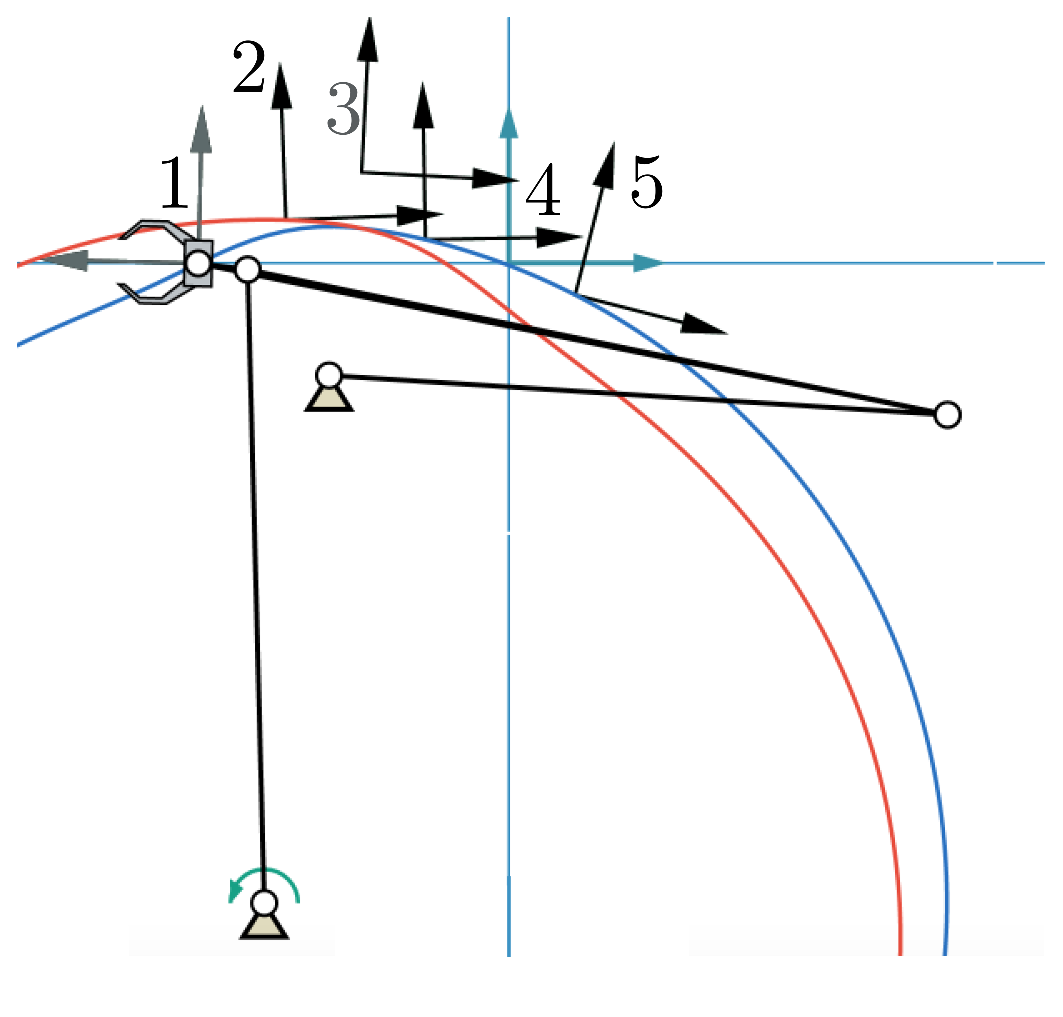
\includegraphics[width=200pt]{jmr-17/figure/fig1.eps}
\caption{Example \ref{5pos}: Optimal four-bar mechanism that minimizes algebraic fitting error for third pose. Although second pose lies on different circuit, this Grashof type four-bar produces desired continuous motion from first to last pose.}
\label{5posgg}
\end{figure}

\subsection{Optimal Linkage for Four Precision Poses with Region Constraint}\label{4pos1line1pose}
\begin{figure}
\centering
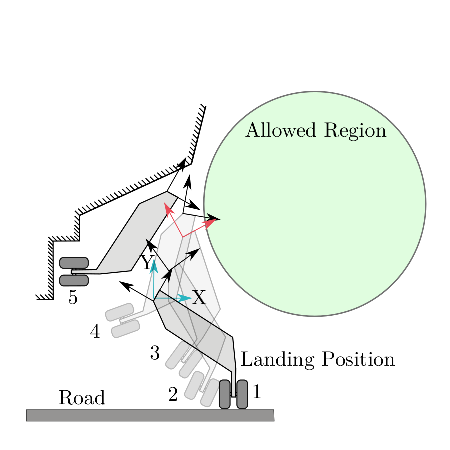
\includegraphics[width=200pt]{jmr-17/figure/fig2.eps}
\caption{Example \ref{4pos1line1pose}: Five landing gear positions are shown where the third position can be relaxed. Allowed region for fixed pivots of mechanism is also shown.}
\label{4posproblem}
\end{figure}

\begin{table}
\caption{Example~\ref{4pos1line1pose}: Pose Data}
\centering
\label{4posMotion}
\begin{tabular}{cccc}
\hline
Poses & X & Y & $\phi$ (degree)\\
\hline
Pose 1 &  -0.0125 & -0.0374 & 66.3 \\
Pose 2 &  0.303 & 0.634 & 35.5 \\
Pose 3 &  0.599 & 1.83 & 352. \\
Pose 4 &  0.268 & 2.30 & 331. \\
Pose 5 &  0.606 & 1.31 & 22.2 \\
\hline
\end{tabular}
\end{table}

\begin{table*}[thb]
  \caption{Example \ref{4pos1line1pose}: Four singular vectors obtained after SVD of the matrix $[A]$ of size $4\times8$. The vectors form basis for the null space}
  \centering
  \begin{tabular}{ccccccccc}
  \hline
  Vector &$p_1$&$p_2$&$p_3$&$p_4$&$p_5$&$p_6$&$p_7$&$p_8$\\
    \hline
   $\textbf{p}_1$& -0.585 & -0.0211 & -0.506 & 0.165 & 0.134 & -0.350 & 0.368 & 0.313 \\
   $\textbf{p}_2$& 0.0640 & -0.330 & 0.190 & -0.804 & 0.236 & -0.264 & 0.194 & 0.204 \\
   $\textbf{p}_3$& -0.280 & 0.0484 & -0.466 & -0.398 & 0.232 & 0.603 & -0.136 & -0.329 \\
   $\textbf{p}_4$& -0.137 & 0.145 & 0.469 & 0.250 & 0.747 & 0.229 & 0.259 & 0.0111 \\
    \hline
  \end{tabular}
  \label{svectors4pos}
\end{table*}

\begin{table*}[thb]
 \caption{Example \ref{4pos1line1pose}: Four optimum dyad-vectors obtained as result of optimization}
  \centering
  \begin{tabular}{ccccccccc}
  \hline
  Vector &$p_1$&$p_2$&$p_3$&$p_4$&$p_5$&$p_6$&$p_7$&$p_8$\\
    \hline
$\textbf{s}_1$&  0.0254 & 0.192 & -0.202 & -0.0965 & 0.00562 & 0.723 & -0.387 & -0.490 \\
$\textbf{s}_2$& 0.276 & -0.406 & 0.211 & -0.425 & -0.161 & -0.561 & 0.251 & 0.360 \\
$\textbf{s}_3$& 0.315 & -0.356 & 0.189 & -0.397 & -0.318 & -0.598 & 0.129 & 0.324 \\
$\textbf{s}_4$& 0.208 & -0.302 & 0.141 & -0.335 & -0.321 & -0.691 & 0.134 & 0.368 \\
    \hline
  \end{tabular}
  \label{dyadvectors4pos}
\end{table*}

Figure~\ref{4posproblem} shows five positions of a landing gear moving from the landing position to the retracted position. Table~\ref{4posMotion} contains position and orientation data for five poses. It is desirable that fixed pivots should lie inside the circle of radius 2.3 with center located at (3.33, 2.04). The task is to synthesize a mechanism which interpolates through precision poses (1,2,4,5) and minimizes the algebraic error for the third pose while keeping fixed pivot locations inside the allowed region as shown in the figure.

First step is to extract all four geometric constraints, i.e. four precision poses and form matrix $[A]$  using Eq.~\req{A8}. Here $n = 4$ which means solution space consists of 4 singular vectors which are obtained using SVD and tabulated in Table~\ref{svectors4pos}. Once this linear algebraic fitting is done, optimization problem can be formulated.

The error function is linear error function $f_1$ for third pose, which is evaluated using Eq.~\req{poseError}. Substituting singular vectors into dyad coefficients followed by substituting them in terms of $\alpha_i$ using Eq.~\req{solutionSpace}, we get final objective function given by
\begin{equation}
f = f_1^2,
\end{equation}
where $f_1 = -0.0598 {\alpha_2}+0.0294 {\alpha_3}-0.100 {\alpha_4}+0.0876$.
The circular region for fixed pivots is modeled as an inequality constraint using Eq.~\req{ellipseIneq} and~\req{g} given by,
\begin{equation}
\begin{array}{c}
g = 0.091 {\alpha_2}^2+(0.25 {\alpha_3}+0.11 {\alpha_4}+0.25) {\alpha_2}\\+0.35 {\alpha_3}^2+0.049 {\alpha_4}^2+{\alpha_3} (0.043 {\alpha_4}+1.0)\\-0.048 {\alpha_4}-0.19 \leq 0
\end{array}
\end{equation}
Objective function also has two quadratic equality constraints given by,
\begin{eqnarray}
& & h_1 = 0.058 {\alpha_2}^2+(-0.25 {\alpha_3}+0.17 {\alpha_4}-0.36) {\alpha_2} -0.34 {\alpha_3}^2  \nonumber \\
& & \ \ \ \ \ \ \ \ \  -0.041 {\alpha_4}^2+{\alpha_3} (0.23 {\alpha_4}-0.38)-0.033 {\alpha_4}+0.29, \nonumber \\
& & h_2  = -0.29 {\alpha_2}^2+{\alpha_2} (-0.15 {\alpha_3}-0.074 {\alpha_4}-0.048)+0.20 {\alpha_3}^2 \nonumber \\
& & \ \ \ \ \ \ \ \ \  +{\alpha_3} (0.18 {\alpha_4}+0.12)-0.46 {\alpha_4}^2-0.11 {\alpha_4}-0.36 \nonumber \\
\end{eqnarray}
We follow steps presented in section~\ref{lagrangeMultiplier} and form Lagrange objective function $F$ given by,
\begin{equation}
F = -{f_1}^2- \lambda_1h_1 -  \lambda_2h_2 - \mu g
\end{equation}
and obtain equations by partial differentiation as well as equation corresponding to Karush-Kuhn-Tucker condition as follow:

\begin{equation}
\begin{array}{c}
\frac{\partial}{\partial \alpha_2}(F) = 0 = (-0.12 {\alpha_2}+0.25 {\alpha_3}-0.17 {\alpha_4}+0.36) {\lambda_1}+(0.57 {\alpha_2}\\+0.15 {\alpha_3}+0.074 {\alpha_4}+0.048) {\lambda_2}-(0.18 {\alpha_2}) \mu \\-(0.25 {\alpha_3}) \mu -(0.11 {\alpha_4}) \mu -0.25 \mu +0.060
\end{array}
\end{equation}

\begin{equation}
\begin{array}{c}
\frac{\partial}{\partial \alpha_3}(F) = 0 = {\lambda_1} (0.25 {\alpha_2}+0.69 {\alpha_3}-0.23 {\alpha_4}+0.38)+{\lambda_2}\\ (0.15 {\alpha_2}-0.41 {\alpha_3}-0.18 {\alpha_4}-0.12)-0.25 {\alpha_2} \mu\\ -0.71 {\alpha_3} \mu -0.043 {\alpha_4} \mu -1.0 \mu -0.029
\end{array}
\end{equation}

\begin{equation}
\begin{array}{c}
\frac{\partial}{\partial \alpha_4}(F) = 0 = {\lambda_1} (-0.17 {\alpha_2}-0.23 {\alpha_3}+0.081 {\alpha_4}+0.033)\\+{\lambda_2} (0.074 {\alpha_2}-0.18 {\alpha_3}+0.92 {\alpha_4}+0.11)-0.11 {\alpha_2} \mu\\ -0.043 {\alpha_3} \mu -0.097 {\alpha_4} \mu +0.048 \mu +0.10
\end{array}
\end{equation}

\begin{equation}
\begin{array}{c}
\frac{\partial}{\partial \lambda_1}(F) = 0 =-0.058 \alpha_2^2+(0.25 \alpha_3-0.17 \alpha_4+0.36) \alpha_2\\+0.34 \alpha_3^2+0.041 \alpha_4^2+\alpha_3 (0.38-0.23 \alpha_4)+0.033 \alpha_4-0.29
\end{array}
\end{equation}

\begin{equation}
\begin{array}{c}
\frac{\partial}{\partial \lambda_2}(F) = 0 =0.29 \alpha_2^2+(0.15 \alpha_3+0.074 \alpha_4+0.048) \alpha_2\\-0.20 \alpha_3^2+0.46 \alpha_4^2+\alpha_3 (-0.18 \alpha_4-0.12)+0.11 \alpha_4+0.36
\end{array}
\end{equation}

\begin{equation}
\begin{array}{c}
\mu\frac{\partial}{\partial \mu}(F) = 0 =\mu(-0.091 \alpha_2^2+(-0.25 \alpha_3-0.11 \alpha_4-0.25) \alpha_2\\-0.35 \alpha_3^2-0.049 \alpha_4^2+\alpha_3 (-0.043 \alpha_4-1.0)+0.048 \alpha_4+0.19)
\end{array}
\end{equation}

Solving these equations followed by filtering on the basis of feasibility using Eq.~\ref{kkt2} yields four unique and feasible solutions tabulated in Table~\ref{alphasol}. All of these solutions satisfy Karush-Kuhn-Tucker Condition for optimality given by Eq.~\req{kkt3}. Dyad vectors are calculated by substituting these solutions into \req{solutionSpace} and are given in Table ~\ref{dyadvectors4pos}. Any of these four dyad-vectors when substituted in Eq.~\req{general} forms a quartic equation, which when projected on hyperplane $Z_4 = 1$ represents a quadric surface. Fig.~\ref{4posmanifolds} shows intersection of hyperboloid and hyperbolic paraboloid  formed from first and second dyad-vectors. The intersection curve represents workspace of the corresponding four-bar linkage. Table~\ref{error4pos} contains the minimized algebraic fitting error of objective function. From this table, we can see that dyad $\textbf{s}_4$ has least pose fitting error. All dyads except $\textbf{s}_1$ are of RR type dyads while $\textbf{s}_1$ is an RP dyad. Figure~\ref{4posRRRP} shows a branch defect free four-bar mechanism formed by combining $\textbf{s}_1$ and $\textbf{s}_2$.

\begin{table}
\caption{Real Solutions for $\alpha_i$, $\lambda_i$ and $\mu$}
\centering
\label{alphasol}
\begin{tabular}{cccccccc}
\hline
Dyad &$\alpha_1$&$\alpha_2$ & $\alpha_3$& $\alpha_4$& $\lambda_1$& $\lambda_2$& $\mu$\\
\hline
$\textbf{s}_1$  & 1 & -0.40 & -0.027 & 1.09 & 0.0 & 0.0 & 0.0 \\
$\textbf{s}_2$ & 1 &  -2.04 & -1.81 & 2.06 & 0.0 & 0.0 & 0.0 \\
$\textbf{s}_3$ & 1 &-3.64 & -4.24 & 5.37 & 0.0 & 0.0 & 0.0 \\
$\textbf{s}_4$ & 1 & 5.08 & -2.58 & -2.94  & 0.0 & 0.0 & 0.0 \\
\hline
\end{tabular}
\end{table}

\begin{table}
\caption{Optimality Evaluations for Dyads}
\centering
\label{error4pos}
\begin{tabular}{ccc}
\hline
Dyad & $3^{rd}$Pose-Fitting Error & Inequality Constraint \\
\hline
$\textbf{s}_1$ &  0.0102 & -0.000650 \\
$\textbf{s}_2$ &  0.0415 & -0.00126 \\
$\textbf{s}_3$ &  0.0212 & -0.000424 \\
$\textbf{s}_4$ & -1.8$\times10^{-8}$ &  -0.396 \\
\hline
\end{tabular}
\end{table}

\begin{figure}
\centering
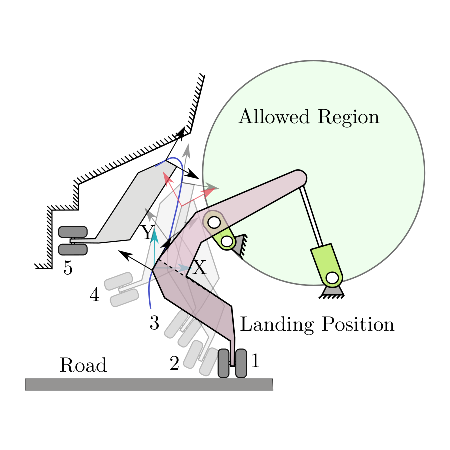
\includegraphics[width=200pt]{jmr-17/figure/fig3.eps}
\caption{Example \ref{4pos1line1pose}: First and second dyad in Table ~\ref{dyadvectors4pos} are combined to form the linkage shown. It can be clearly seen that coupler curve fairly approximates the third pose while fixed pivots are inside the allowed region.}
\label{4posRRRP}
\end{figure}

\begin{figure}
\centering
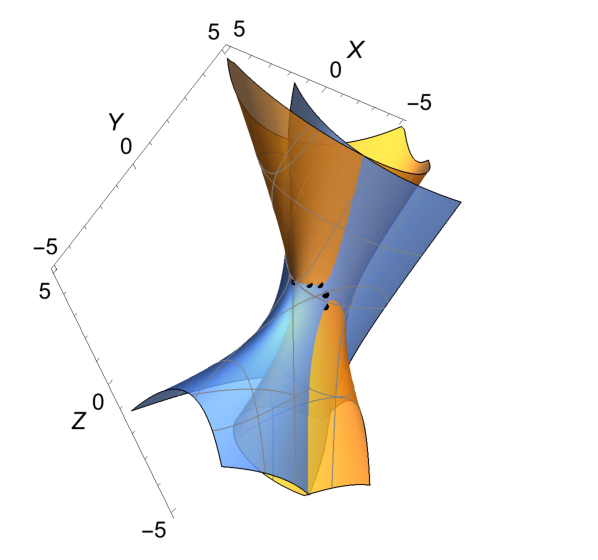
\includegraphics[width=200pt]{jmr-17/figure/fig4.eps}
\caption{Example \ref{4pos1line1pose}: Image-Space representation of intersection of third and fourth optimal constraint manifolds from Table.~\ref{dyadvectors4pos}. Also shown are five image points as dark spheres representing the five poses; four of them lie exactly on the intersection of the two surfaces, while one is closest possible.}
\label{4posmanifolds}
\end{figure}

\section{Conclusion}
In this chapter, we presented a task-driven approach to unified and optimal synthesis of planar four-bar linkages for extended Burmester problem. In this formulation, various geometric constraints are treated equivalently, which in turn leads to a much simpler two-step based algorithm for computing planar dyads of four-bar linkages. Original contributions of this chapter have been into reforming a mixed exact-approximate algebraic fitting problem into problem of task oriented optimal fitting of algebraic manifold. The framework presented here can accommodate linear as well as non-linear equality and inequality geometric constraints and minimize objective functions that can be expressed in terms of dyadic parameters. Although adding non-linear geometric constraints increase computational complexity, computer algebra software like Mathematica could be used to compute solutions of quadratic system of equations in a reasonable amount of time. Experimentations show that Mathematica takes less than 3 seconds on a MacBook Pro with 2.4GHz Intel core i5 processor and 8GB RAM for computing solutions for the system of seven quadratic equations. The framework also preserves previously achieved real-time solutions for linear geometric constraints with no optimality criterion. Two examples demonstrating computation of optimal type and dimensions of dyads that minimize task oriented objective function are presented.

This work has been published in ASME Journal of Mechanisms and Robotics, 2017~\cite{shrinathpurwar2017}.
